\section{Các tính năng đã hỗ trợ}

Phần này sẽ trình bày một số tính năng khác biệt của Rust so với ngôn ngữ C/C++ và cách mà công cụ đã hỗ trợ cho các tính năng này. Các tính năng bao gồm: if let, while let, match, lifetime.

\subsection{if let}
If else là cấu trúc điều khiển phổ thông có mặt trong tất cả các loại ngôn ngữ phổ biến.
Nó cho phép chúng ta kiểm tra một điều kiện và thực thi một khối mã nếu điều kiện đó đúng và một khối mã khác nếu điều kiện đó sai.
Cấu trúc câu lệnh if else sẽ bao gồm một điều kiện và 2 khối mã.
Nếu điều kiện đúng, khối mã trong if sẽ được thực thi, ngược lại khối mã trong else sẽ được thực thi.
Thông thường khối điều kiện sẽ là biểu thức trả về kết quả đúng hoặc sai của biểu thức đó.
Trong ngôn ngữ như C/C++ thì chỉ chấp nhận biểu thức điều kiện, sử dụng mệnh đề điều kiện sử dụng dấu hai chấm kết thúc câu lệnh là không hợp lệ.

Rust với tinh thần \textit{"Expression over statement"} và nhằm mục đích tạo sự ngắn gọn cho câu lệnh, Rust cho phép thực hiện phép khai báo biến và gán giá trị cho biến trong cùng một câu lệnh điều kiện if.
Cú pháp của câu lệnh if let

\usemintedstyle{bw}

\begin{minted}[mathescape, breaklines, frame=lines, framesep=2mm, baselinestretch=1.2, fontsize=\footnotesize, linenos]{rust}
if let <pattern> = <expression> {
     <block>
} else {
     <block>
}
\end{minted}

\usemintedstyle{default}

Cú pháp này sẽ thực hiện 2 công việc, kiểm tra xem $<expression>$ có match với $<pattern>$ hay không, nếu không match thì trả về $false$, nếu có match thì tiếp tục thực hiện tạo biến mới dựa theo $<pattern>$ vừa lấy được. Các biến lấy được từ $<pattern>$ sẽ có phạm vi tồn tại trong khối lệnh điều kiện thành công của lệnh if. Do thực hiện 2 công việc trong cùng 1 câu lệnh nên khi quy đổi sang câu lệnh tương tự trong ngôn ngữ khác như C/C++ sẽ tương đương 2 câu lệnh gán biến và kiểm tra điều kiện.

\begin{listing}[H]
\begin{minted}[mathescape, breaklines, frame=lines, framesep=2mm, baselinestretch=1.2, fontsize=\footnotesize, linenos]{rust}
let number: Option<i32> = None;
let i_like_letters = false;

if let Some(i) = number {
    println!("Matched number {:?}!", i);
} else if i_like_letters {
    // ...
} else {
    // ...
}
\end{minted}
\caption{Ví dụ mã nguồn cho if let}
\label{code:c4_iflet}
\end{listing}

\begin{listing}[H]
\begin{minted}[mathescape, breaklines, frame=lines, framesep=2mm, baselinestretch=1.2, fontsize=\footnotesize, linenos]{cpp}
Object* obj = inputObj();

if (obj != nullptr) { // 1 câu lệnh kiểm tra điều kiện
    int number = *static_cast<int*>(obj); // 1 câu lệnh gán biến
    std::cout << "Matched " << number << "!" << std::endl;
}
\end{minted}
\caption{Ví dụ mã nguồn cho if let tương đương trong C++}
\label{code:c4_iflet_cpp}
\end{listing}

Trong hình \ref{img:c4_cpg_iflet}, cạnh CONDITION của nút ExprIf trỏ tới nút Local, đồng thời cũng khai báo biến mới với tên $i$. Các mệnh đề trong khối code được thực thi khi điều kiện đúng nếu có nhắc tới biến $i$ thì sẽ tham chiếu tới biến $i$ vừa được khai báo thông qua cạnh REF.

\begin{figure}[H]
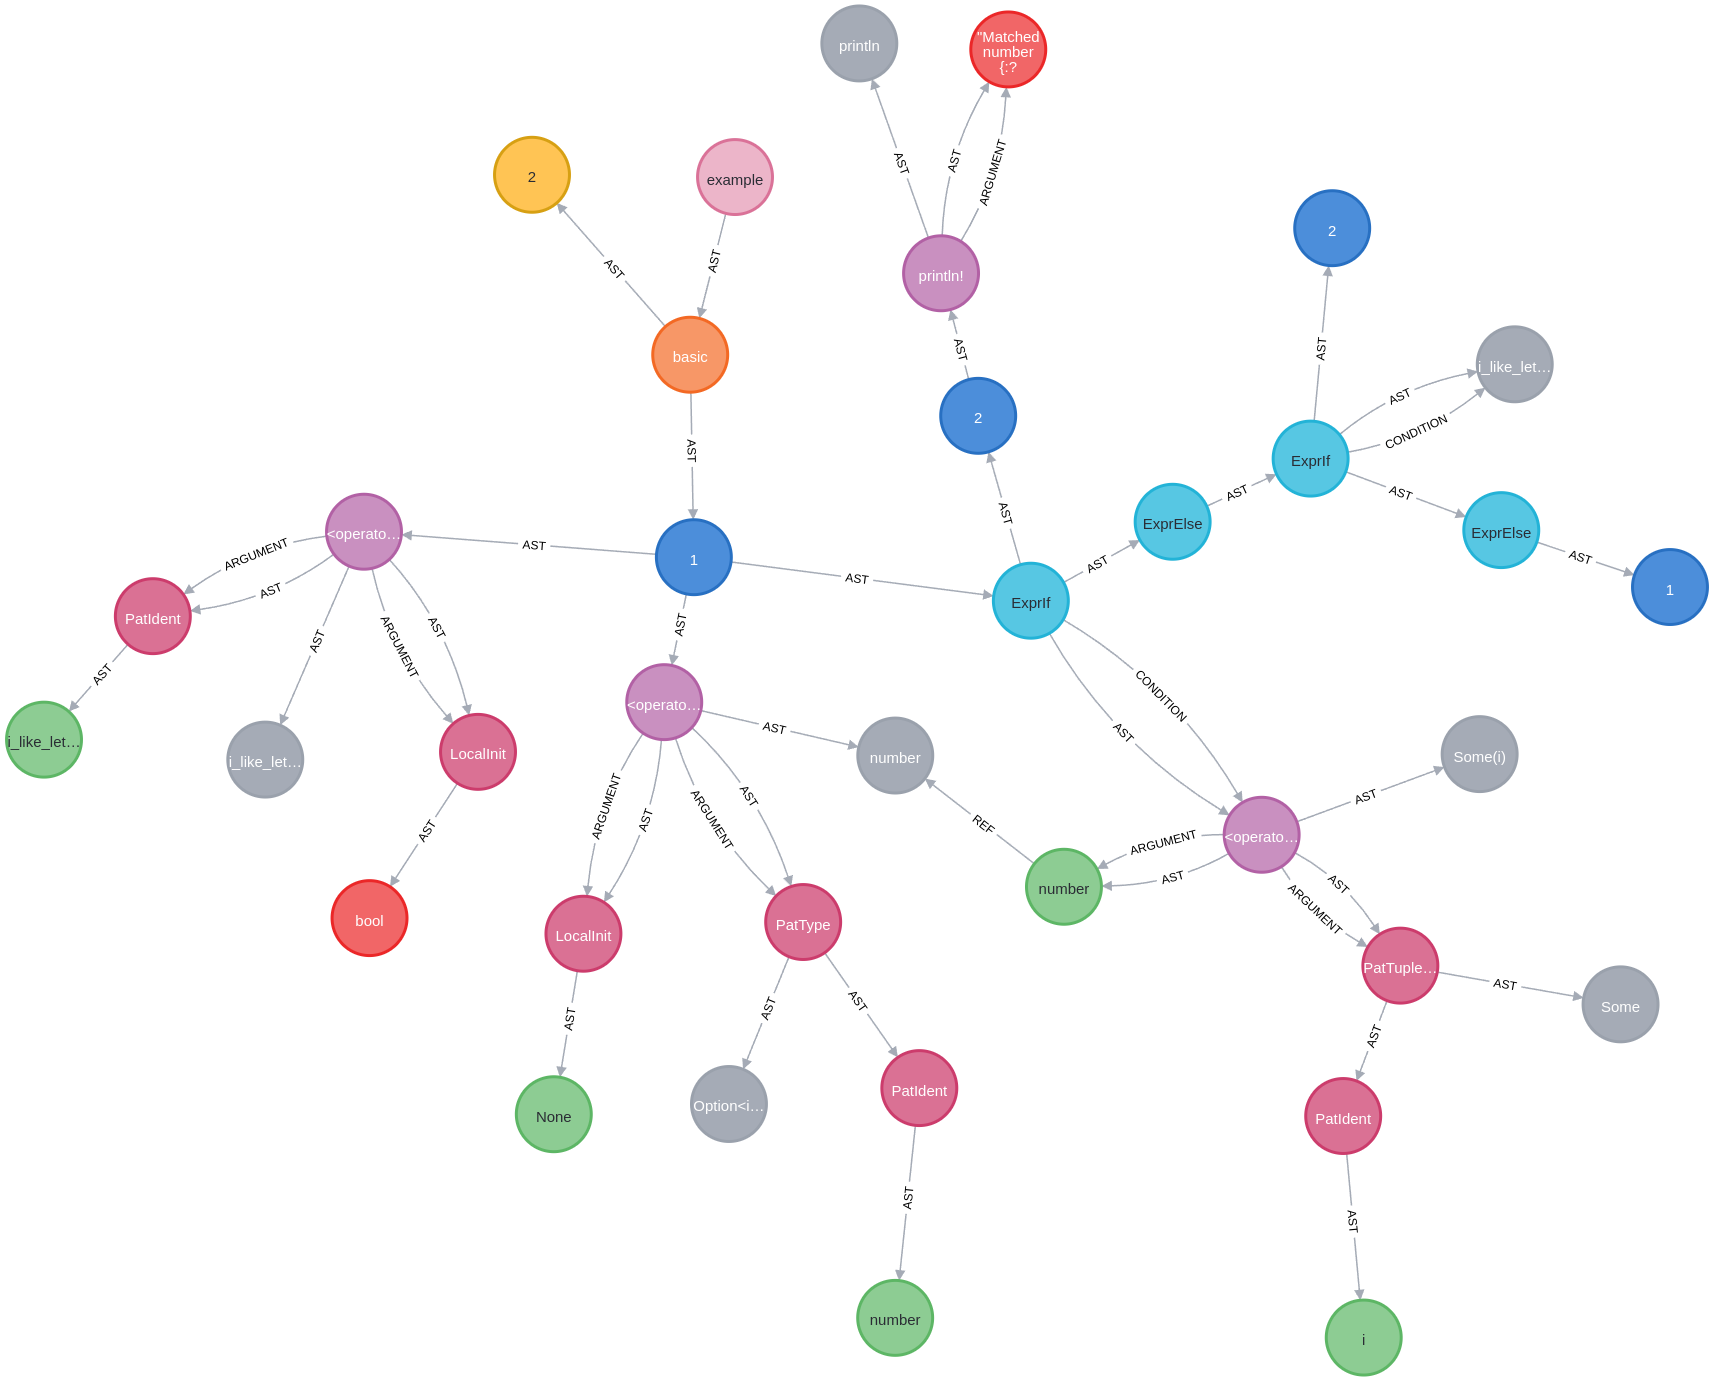
\includegraphics[width=1\columnwidth]{figures/c4/c4_iflet.png}
\centering
\caption{Ví dụ đồ thị thuộc tính mã nguồn cho đoạn mã nguồn if let \ref{code:c4_iflet}}
\label{img:c4_cpg_iflet}
\end{figure}

\subsection{while let}

Tương tự với tính năng if let ở trên, Rust cũng hỗ trợ việc khai báo biến làm điều kiện cho vòng lặp while.
Có thể hiểu là nếu việc match với pattern của vế trái thành công thì sẽ tiếp tục thực hiện vòng lặp, sẽ có 1 biến $i$ mới được khởi tạo đối với mỗi lần lặp.
Các mệnh đề trong khối code khi điều kiện thành công của vòng lặp sẽ tham chiếu tới biến $i$ vừa được khai báo thông qua cạnh $REF$ nếu có sử dụng tới.
Không chỉ vậy vế phải của điều kiện có thể được gán lại liên tục trong quá trình lặp, nếu vế trái không match với pattern nào thì vòng lặp sẽ kết thúc.

\begin{listing}[H]
\begin{minted}[mathescape, breaklines, frame=lines, framesep=2mm, baselinestretch=1.2, fontsize=\footnotesize, linenos]{rust}
let mut optional = Some(0);

while let Some(i) = optional {
    if i > 9 {
        println!("Greater than 9, quit!");
        optional = None;
    } else {
        println!("`i` is `{:?}`. Try again.", i);
        optional = Some(i + 1);
    }
}
\end{minted}
\caption{Ví dụ mã nguồn cho while let}
\label{code:c4_whilelet}
\end{listing}

\begin{figure}[H]
    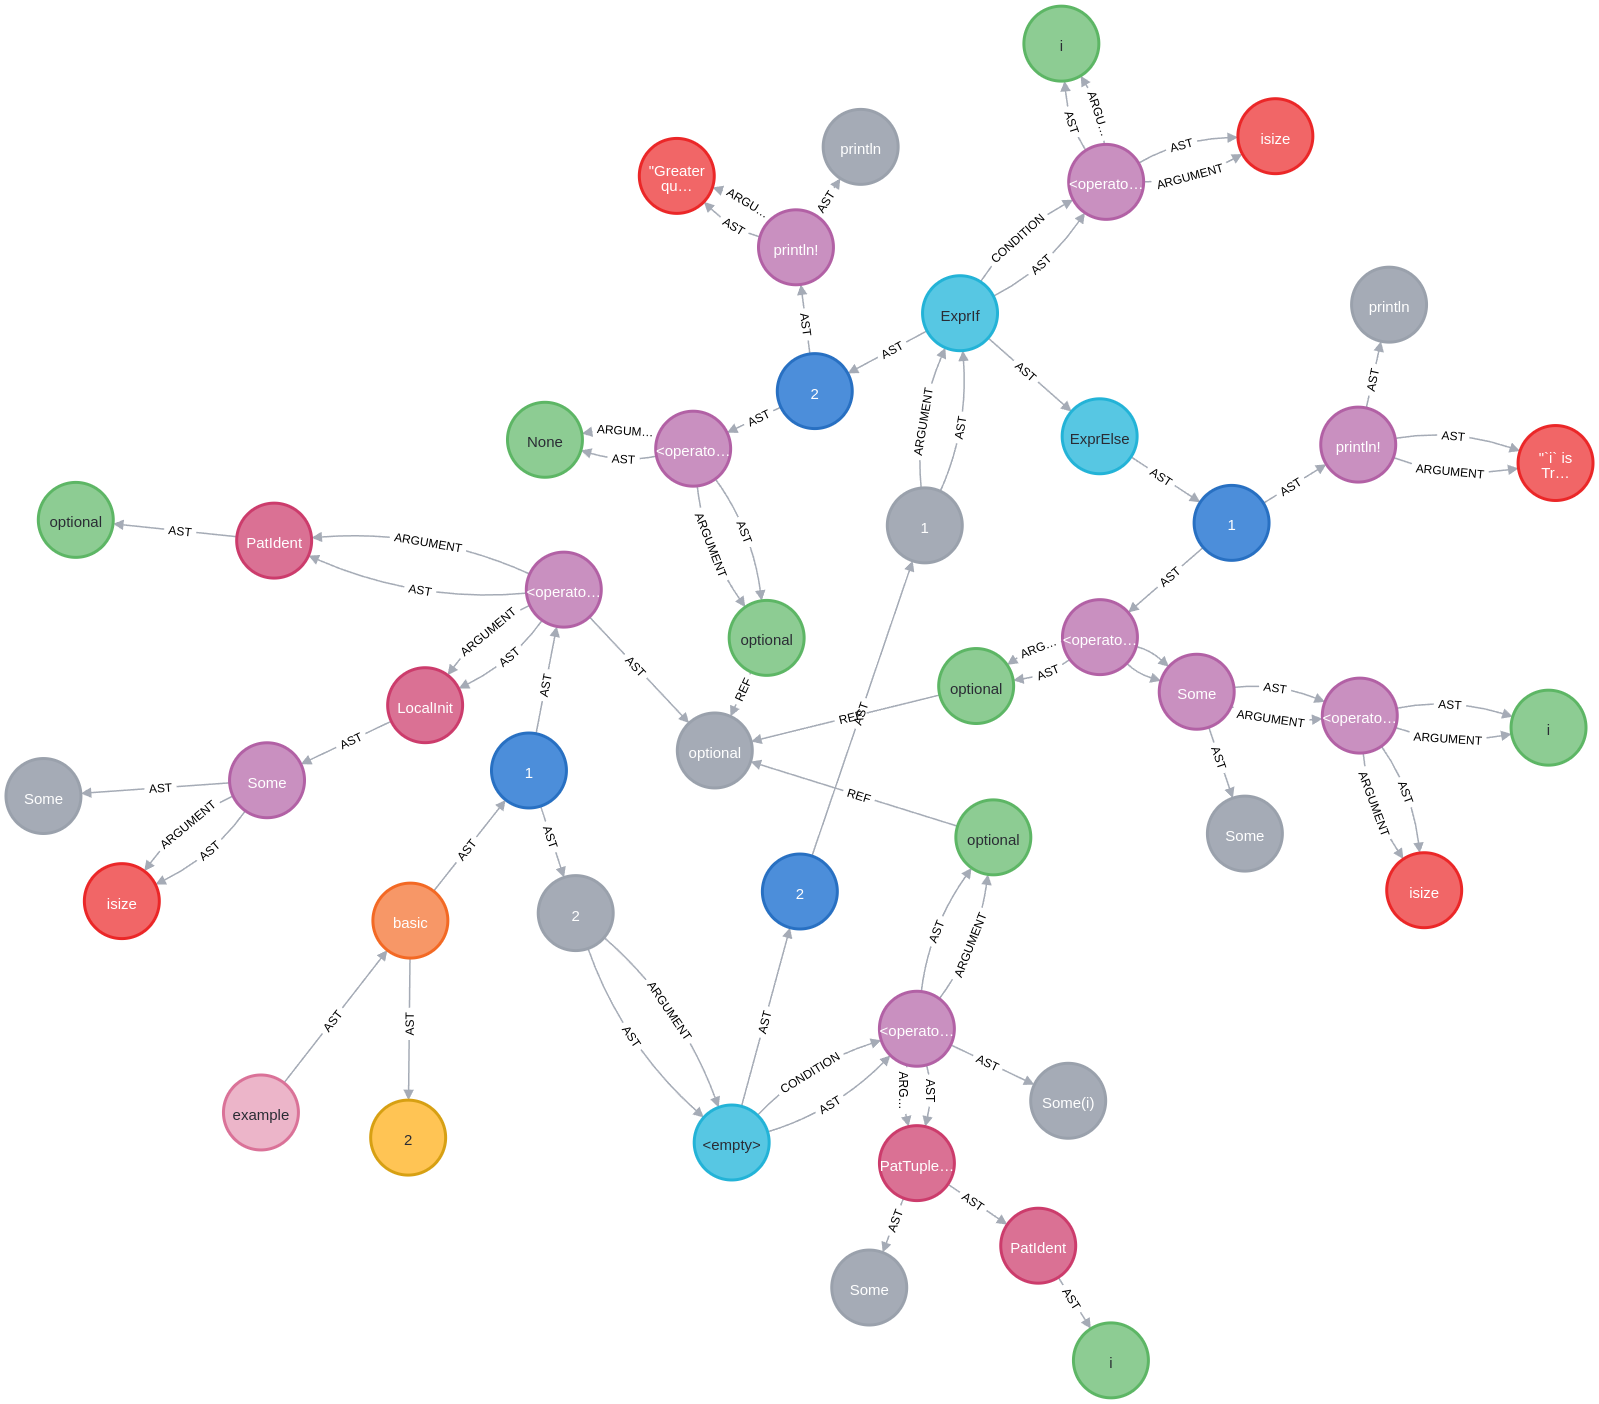
\includegraphics[width=1\columnwidth]{figures/c4/c4_whilelet.png}
    \centering
    \caption{Ví dụ đồ thị thuộc tính mã nguồn cho đoạn mã nguồn while let \ref{code:c4_whilelet}}
    \label{img:c4_cpg_whilelet}
\end{figure}

\subsection{match}

Ngoài việc có thể sử dụng mệnh đề gán biến thành biểu thức điều kiện, tính hướng hàm của Rust còn thể hiện ở tính năng match, sự kết hợp giữa pattern matching và Algebraic Data Types.
Cấu trúc match không chỉ kiểm tra giá trị mà còn kết hợp với các pattern phức tạp, bao gồm kiểm tra điều kiện, so sánh và kiểm tra các kiểu dữ liệu khác nhau.
Điều này mang lại cho Rust tính linh hoạt cao hơn so với switch trong C/C++ khi chỉ so sánh giá trị nguyên thủy.

Một điểm khác biệt quan trọng giữa match và switch là tính toàn diện của match. Rust yêu cầu các pattern trong match phải bao quát tất cả các khả năng có thể xảy ra, nếu không trình biên dịch sẽ báo lỗi. Điều này giúp đảm bảo rằng không có tình huống nào bị bỏ qua, tăng cường độ an toàn và độ tin cậy của mã nguồn. Trong khi đó, switch trong C/C++ không yêu cầu bao quát tất cả các trường hợp, và việc bỏ sót một trường hợp có thể dẫn đến lỗi logic hoặc hành vi không mong muốn. Thêm vào đó, match trong Rust cho phép trích xuất và xử lý các thành phần của cấu trúc dữ liệu phức tạp ngay trong quá trình đối chiếu pattern. Ví dụ, Rust có thể match trên các mảng, tuple, enum, struct, trong khi switch của C/C++ thường chỉ giới hạn trong các giá trị nguyên thủy.

\begin{listing}[H]
\begin{minted}[mathescape, breaklines, frame=lines, framesep=2mm, baselinestretch=1.2, fontsize=\footnotesize, linenos]{rust}
enum Color {
    Red,
    Blue(u32, u32, u32),
    Green { red: u32, green: u32, blue: u32, },
}

fn main() {
    let color = Color::Blue(0, 0, 255);

    match color {
        Color::Red => println!("The color is Red!")
        Color::Blue(r, g, b) => println!("Red: {}, green: {}, and blue: {}!", r, g, b)
        Color::Green {red, green, blue} => println!("Red: {}, green: {}, and blue: {}!", red, green, blue),
    }
}
\end{minted}
\caption{Ví dụ mã nguồn cho match, pattern matching}
\label{code:c4_match}
\end{listing}

\begin{figure}[H]
    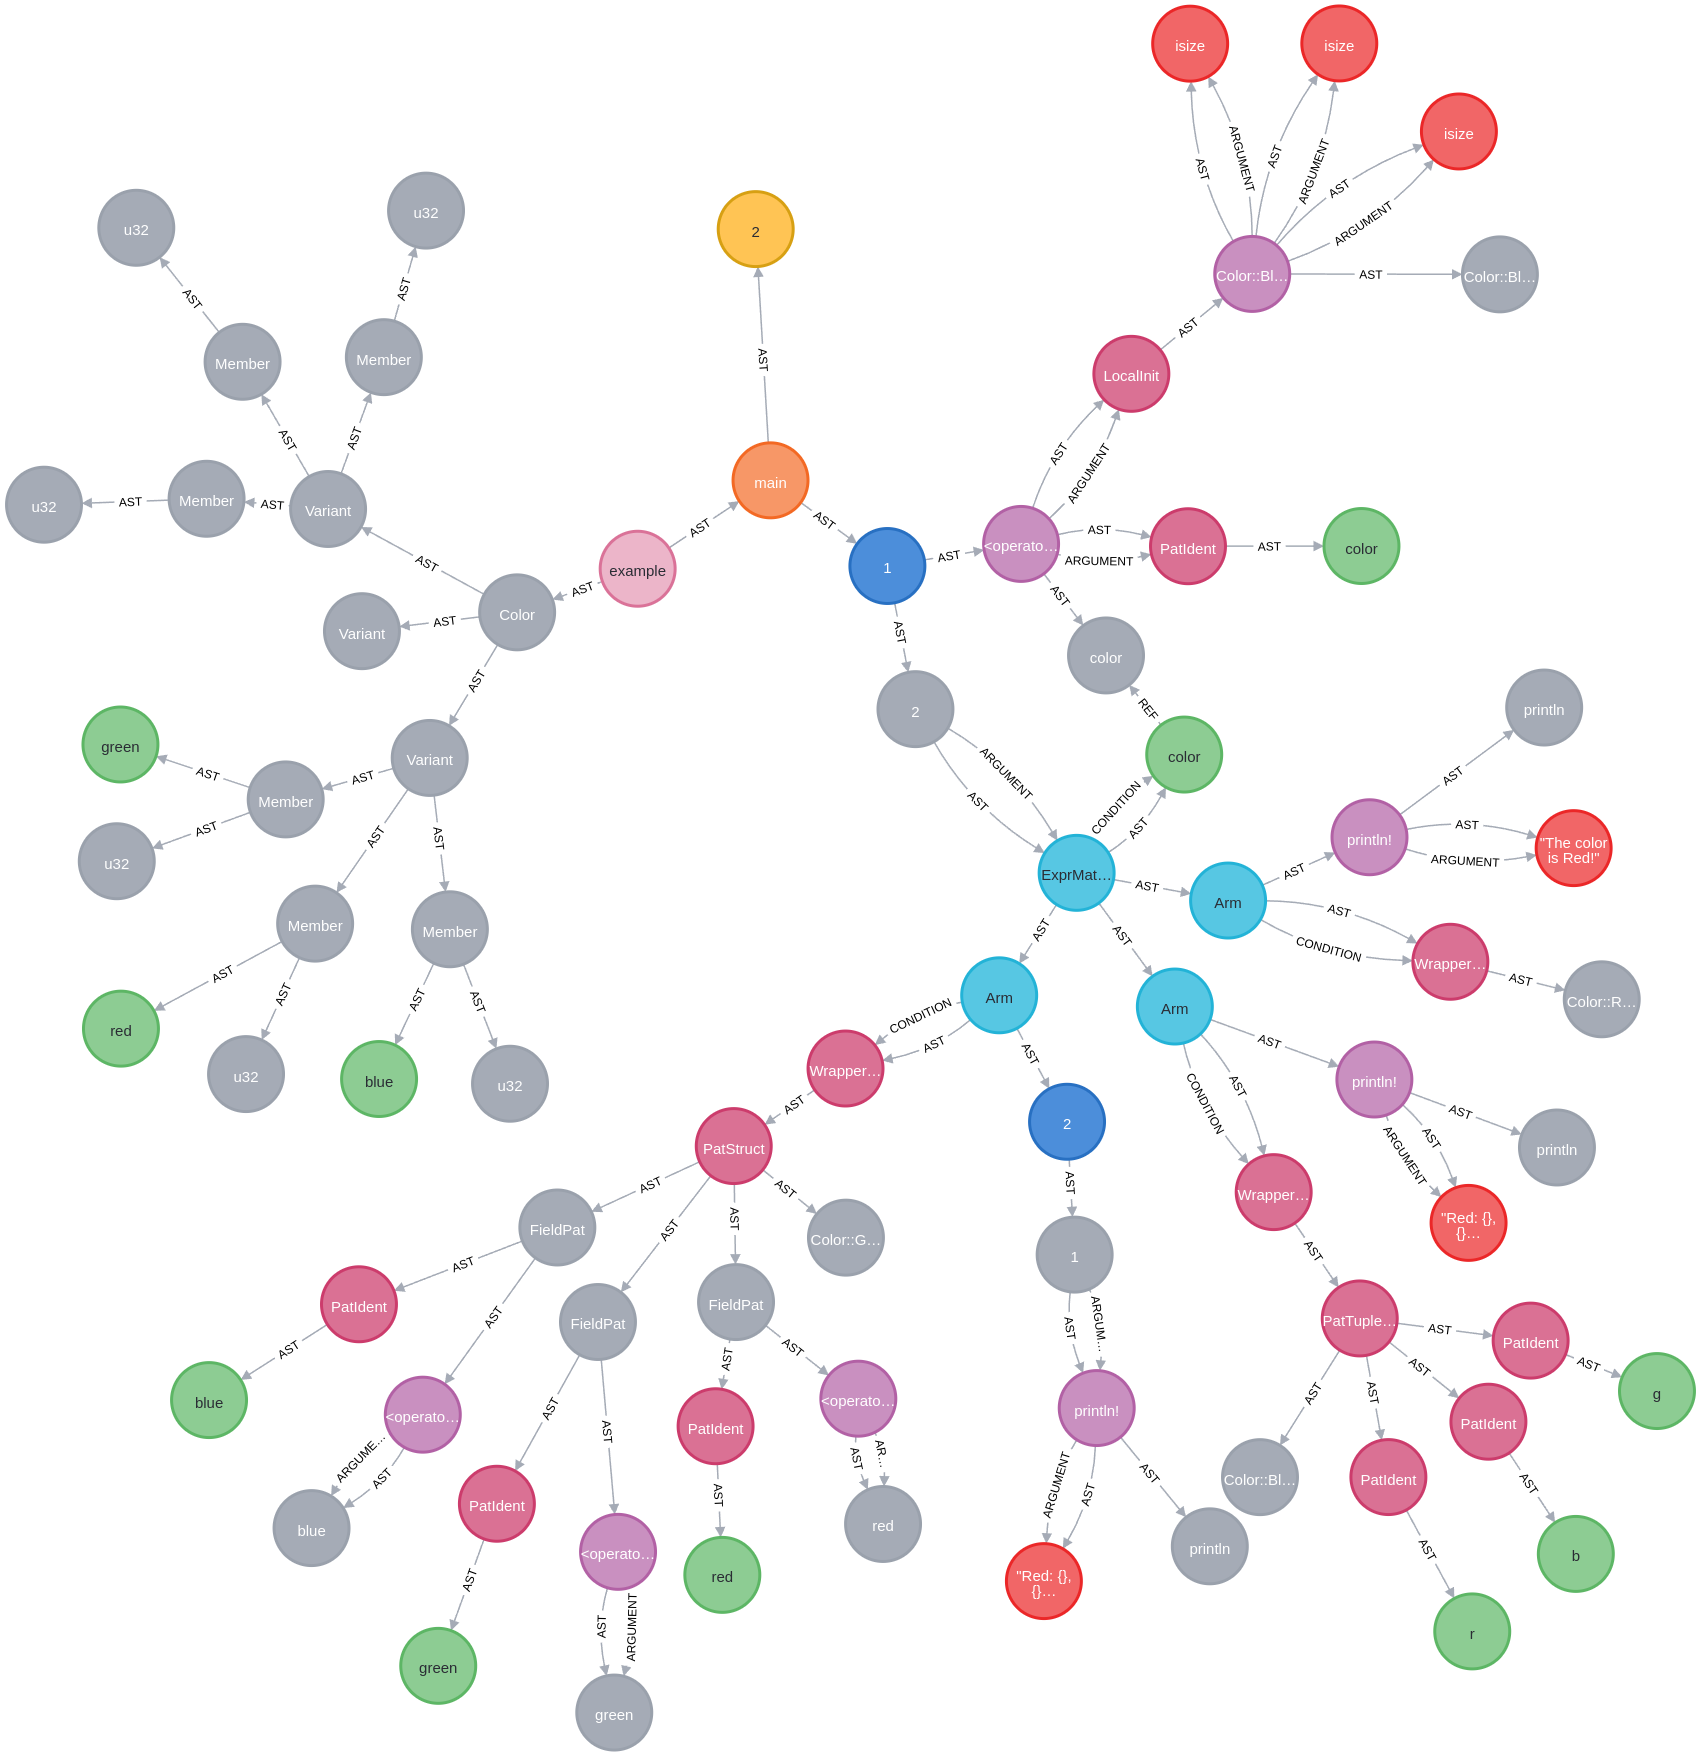
\includegraphics[width=1\columnwidth]{figures/c4/c4_match.png}
    \centering
    \caption{Ví dụ đồ thị thuộc tính mã nguồn cho đoạn mã nguồn match \ref{code:c4_match}}
    \label{img:c4_match}
\end{figure}

\subsection{lifetime}

Lifetime là cơ chế được sử dụng trong Rust để quản lý vòng đời của các biến reference, đảm bảo rằng các biến reference không trỏ tới vùng nhớ không còn tồn tại. Lifetime có vai trò tương tự như Generic Parameter cho biến, nhưng thay vì định kiểu cho biến thì lifetime sẽ xác định vòng đời cho biến reference. Để biểu diễn được tính năng lifetime trên CPG có 3 loại nút mới được thêm vào đặc tả CPG là Lifetime, Lifetime Parameter, Lifetime Argument.
Ngoài ra còn có cạnh OUT\_LIVE được bổ sung để chỉ ra quan hệ giữa biến và lifetime, quan hệ giữa các lifetime với nhau.

Lifetime Parameter và Lifetime Argument được sử dụng cho các hàm, struct, enum, trait để chỉ ra tham số tổng quát về vòng đời cho các biến tham chiếu. Loại nút Lifetime sẽ thể hiện vòng đời thực sự của biến reference. Các biến reference sẽ được gán lifetime thông qua cú pháp 'a, 'b, 'c, ... Nếu các biến cùng đánh dấu lifetime 'a thì sẽ có cạnh OUT\_LIVE trỏ từ biến tới nút đại diện cho 'a tương ứng. Nếu lifetime 'a được giới hạn bởi lifetime 'b thì sẽ có cạnh OUT\_LIVE từ nút Lifetime 'a tới nút Lifetime 'b.

Ownership, borrow checker và lifetime là 3 tính năng làm nên cơ chế an toàn về bộ nhớ trong Rust. Do vậy CPG phải thể hiện được 3 tính năng trên đồ thị và cung cấp các thông tin thông qua các nút, cạnh và thuộc tính phù hợp. Đặc biệt là tính năng lifetime, vòng đời hợp lệ của các biến được thể hiện qua lifetime do đó việc thể hiện đúng quan hệ giữa lifetime và biến, lifetime với lifetime, biến với biến là rất quan trọng. Từ đó có thể khai thác thông tin để kiểm tra vòng đời của biến reference, giúp phát hiện được các lỗi về bộ nhớ vô tình gây ra khi đánh dấu lifetime không chính xác.

% Lifetime elision là một cơ chế trong Rust giúp đơn giản hóa việc viết mã bằng cách tự động suy luận lifetime cho các biến reference. Có ba luật chính về lifetime elision trong Rust. Thứ nhất, nếu một hàm chỉ có một biến reference đầu vào, Rust sẽ tự động gán lifetime cho biến đó mà không cần phải ghi rõ. Thứ hai, nếu một hàm có nhiều hơn một biến reference đầu vào nhưng chỉ có một biến reference đầu ra, Rust sẽ suy luận rằng biến reference đầu ra có cùng lifetime với một trong các biến reference đầu vào. Cuối cùng, nếu một hàm có nhiều hơn một biến reference đầu vào và nhiều hơn một biến reference đầu ra, Rust yêu cầu phải ghi rõ lifetime cho tất cả các biến reference để tránh nhầm lẫn và đảm bảo an toàn bộ nhớ.

% Nói về 3 luật Lifetime Ellision trong Rust, nếu có thể suy luận được lifetime thì không cần phải ghi rõ lifetime, nếu không thể suy luận được thì phải ghi rõ lifetime, nếu có nhiều hơn 1 biến reference thì phải ghi rõ lifetime

\begin{listing}[H]
\begin{minted}[mathescape, breaklines, frame=lines, framesep=2mm, baselinestretch=1.2, fontsize=\footnotesize, linenos]{rust}
fn longest<'a>(x: &'a str, y: &'a str) -> &'a str {
    if x.len() > y.len() {
        x
    } else {
        y
    }
}
\end{minted}
\caption{Ví dụ mã nguồn cho lifetime cho hàm}
\label{code:c4_lifetime_1}
\end{listing}

\begin{figure}[H]
    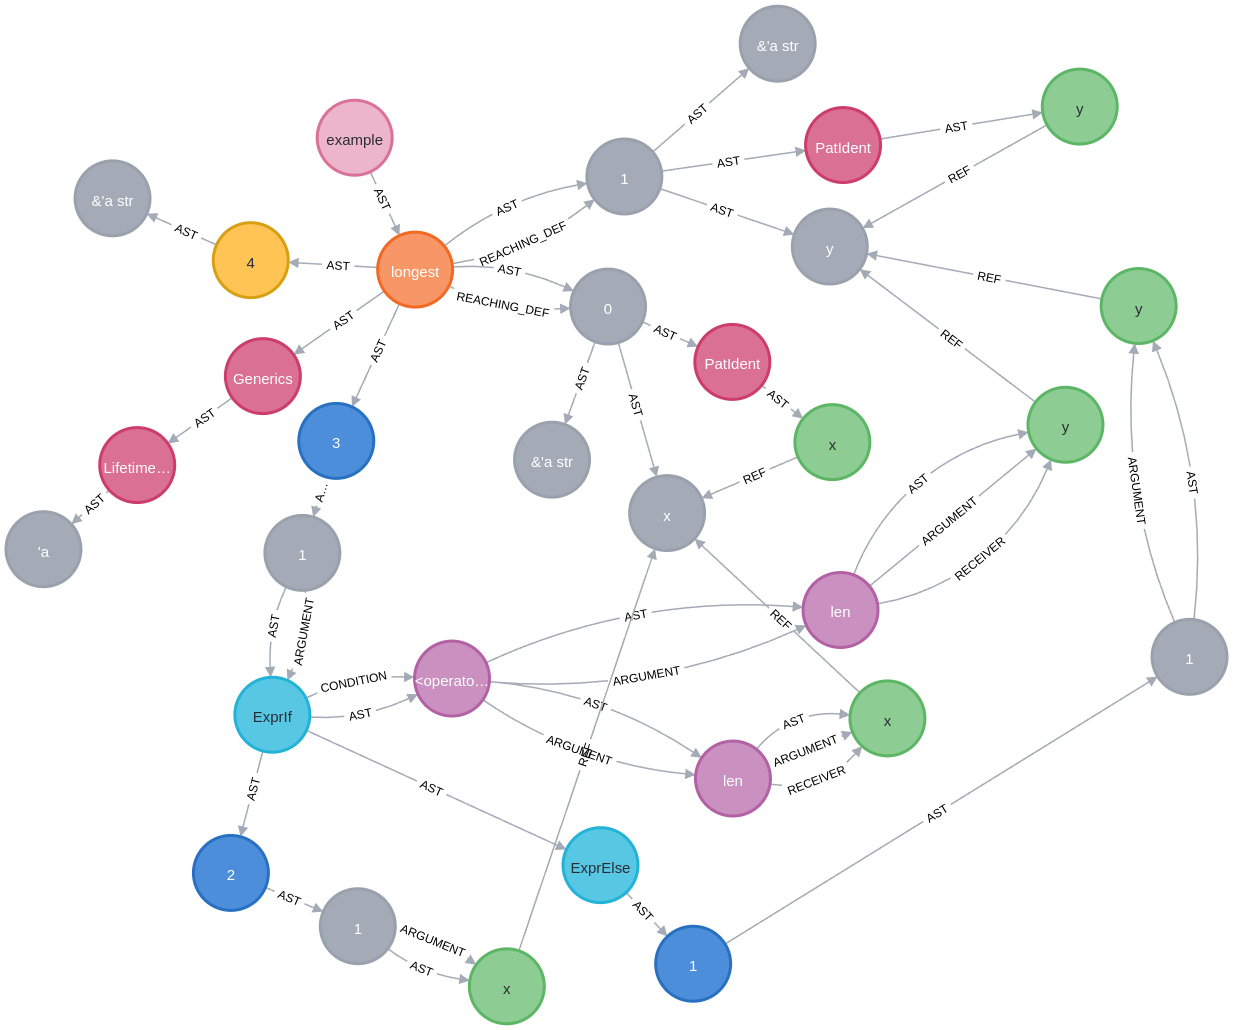
\includegraphics[width=1\columnwidth]{figures/c4/c4_lifetime_1.png}
    \centering
    \caption{Ví dụ đồ thị thuộc tính mã nguồn cho đoạn mã nguồn \ref{code:c4_lifetime_1}}
    \label{img:c4_lifetime_1}
\end{figure}

\begin{listing}[H]
\begin{minted}[mathescape, breaklines, frame=lines, framesep=2mm, baselinestretch=1.2, fontsize=\footnotesize, linenos]{rust}
fn f<'a, 'b, 'c, 'd: 'c>(x: &'a i32, mut y: &'b i32, z: &'c i32)
where
    'a: 'b,
{
    // ...
}
\end{minted}
\caption{Ví dụ mã nguồn cho giới hạn lifetime}
\label{code:c4_lifetime_2}
\end{listing}

\begin{figure}[H]
    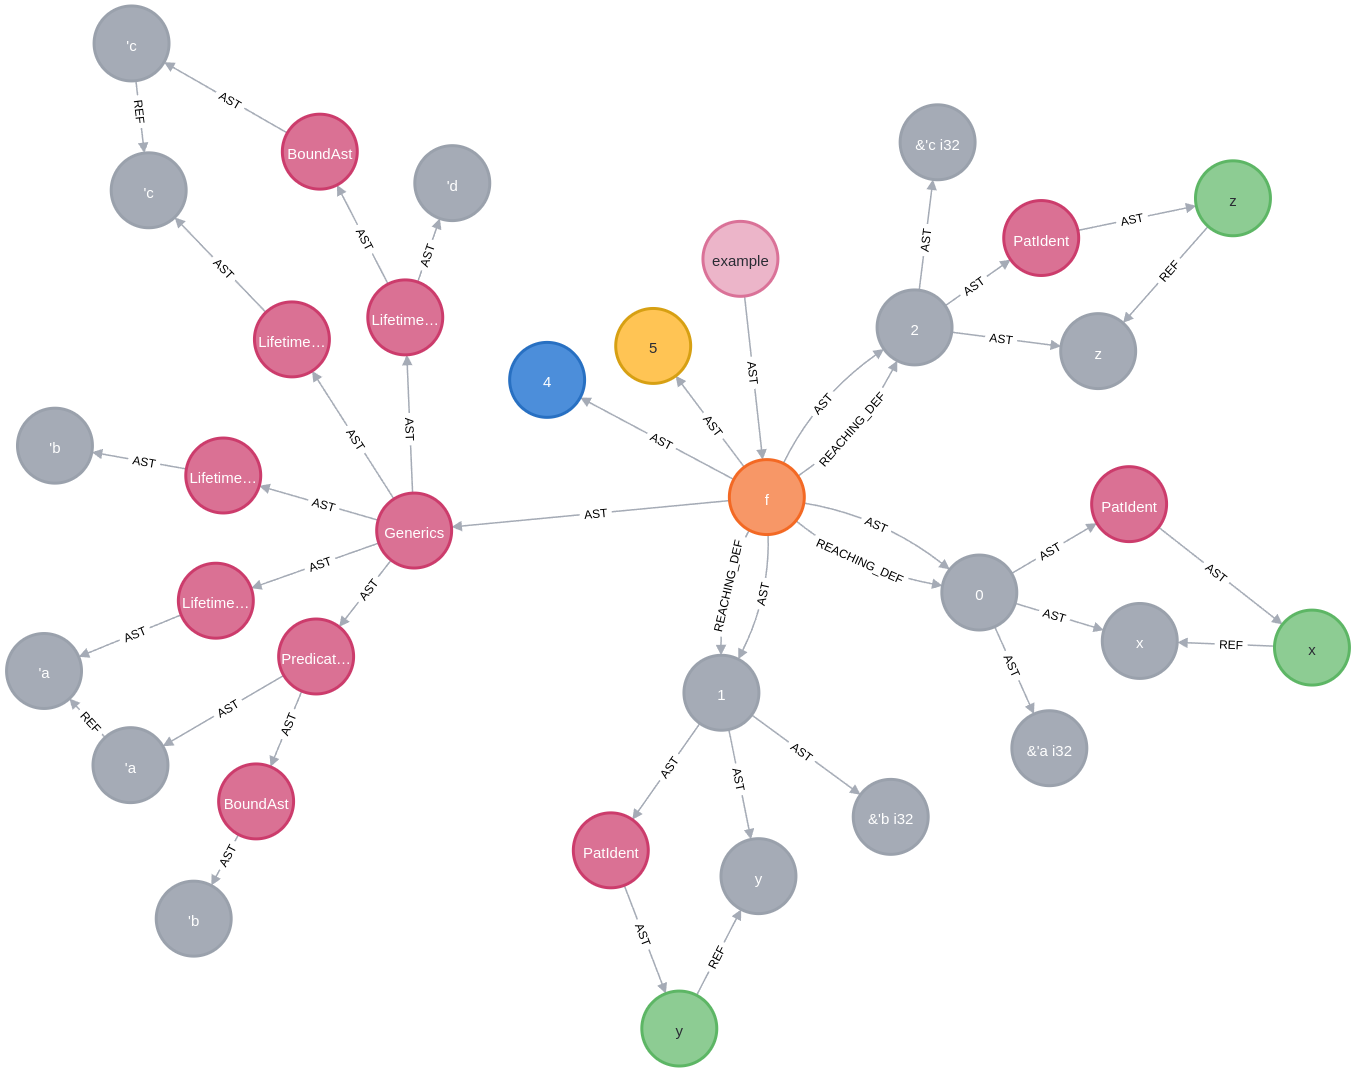
\includegraphics[width=1\columnwidth]{figures/c4/c4_lifetime_2.png}
    \centering
    \caption{Ví dụ đồ thị thuộc tính mã nguồn cho đoạn mã nguồn \ref{code:c4_lifetime_2}}
    \label{img:c4_lifetime_2}
\end{figure}

